\documentclass[10pt,letterpaper]{article}
\usepackage[utf8]{inputenc}
\usepackage{amsmath}
\usepackage{amsfonts}
\usepackage{amssymb}
\usepackage{graphicx}
\usepackage[margin=1in]{geometry}
\author{Yulin Shi, Structure dynamics and vibration laboratory, McGill University}
\title{Harmonic balance method for Duffing oscillators}
\begin{document}
\maketitle
%%%%%%%%%%%%%%%%%%%%%%%% %%%%%%%%%%%%%%%%%%%%%%%% %%%%%%%%%%%%%%%%%%%%%%%% %%%%%%%%%%%%%%%%%%%%%%%% 
\section{Harmonic balance method}
\begin{figure}[ht!]
	\centering
	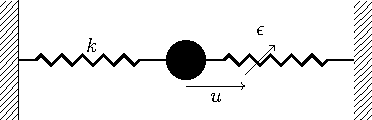
\includegraphics[scale=1]{figure/duff_one_dof/tikz}
	\caption{Duffing oscillator}
	\label{fig:duff_one_dof}
\end{figure}
We are interested in finding the steady solutions of the one degree-of freedom Duffing oscillator under periodic forcing in Figure~\ref{fig:duff_one_dof}
\begin{equation}
	r(t):=m\ddot{u}(t) + \delta \dot{u}(t) + ku(t) + \epsilon u(t)^3 - f(t)
\end{equation}
where $u(t)$ is the unknown displacement variable, $t$ is the time, $f(t)$ is the periodic external forcing. Others are constant coefficients. 

Assume the solutions takes the form of \emph{truncated Fourier series}
\begin{equation}\label{eq:undetermined_coefficients_solution}
	u(t) \approx \frac{a_0}{\sqrt{2}} +\sum_{m=1}^M \cos(m\omega t)a_m+\sin(m\omega t)b_m =\boldsymbol{\phi}(t) \bar{\mathbf u}
\end{equation}
where $\omega$ is the external forcing frequency, and $M$ is the number of harmonics. Array $\bar{\mathbf u}$ stores the unknown coefficients $a_m$ and $b_m$, array $\boldsymbol\phi(t)$ stores the base functions $\cos(m\omega t)$ and $\sin(m\omega t)$. 
Then 
\begin{equation}
	\dot{u}(t) \approx \dot{\boldsymbol{\phi}}(t) \bar{\mathbf u}
,\quad	\ddot{u}(t) \approx \ddot{\boldsymbol{\phi}}(t) \bar{\mathbf u}
\end{equation}

The \emph{Galerkin projection} creates nonlinear equations with respect to $\bar{\mathbf u}$ 
\begin{equation}\label{eq:galerkin_projection}
	\bar{\mathbf r}(\bar{\mathbf u})
	=T^{-1}\int_0^T \boldsymbol\phi^\top (t) r(\ddot{\boldsymbol\phi}(t) \bar{\mathbf u}, \dot{\boldsymbol\phi}(t) \bar{\mathbf u},\boldsymbol\phi(t) \bar{\mathbf u},t) \mathrm dt=\mathbf 0
\end{equation}
where $T=\frac{2\pi}{\omega}$ is the period. It can be solved by the Newton-Raphson method
\begin{equation}
	\bar{\mathbf u}^{(k+1)} \leftarrow \bar{\mathbf u}^{(k)} -(\nabla \bar{\mathbf r}(\bar{\mathbf u}^{(k)}))^{-1} \bar{\mathbf r}(\bar{\mathbf u}^{(k)})
\end{equation}

For Fourier base functions, the integration of the time-variant part in \eqref{eq:galerkin_projection} yields the closed form
\begin{equation}\label{eq:closed_form}
	(m\mathbf L_M + \delta \mathbf L_D + k\mathbf L_K) \bar{\mathbf u} + \frac{1}{N}\sum_{n=1}^N \boldsymbol{\phi}^\top(t_n) \epsilon ( \boldsymbol{\phi}(t_n) \bar{\mathbf u} )^3 - \mathbf L_f= \mathbf 0
\end{equation}
where $N$ is the number of discretized time intervals of one period, $\mathbb R^{2M+1}\times R^{2M+1}$ matrices $\mathbf L_D$ and $\mathbf L_K$ denote respectively
\begin{equation}\label{eq:periodic/hbm_shape_2}
\mathbf L_K := T^{-1} \int_0^{T} \boldsymbol\phi(t)^\top \boldsymbol\phi(t) \mathrm d t
\quad\text{and}\quad
\mathbf L_D := T^{-1} \int_0^{T} \boldsymbol\phi(t)^\top\dot{\boldsymbol\phi}(t) \mathrm d t
\end{equation}
Also, according to the Green equation, $\mathbf L_M$ simplifies as
\begin{equation}\label{eq:periodic/hbm_shape_3}
\mathbf L_M
:= T^{-1} \int_0^{T} \boldsymbol\phi(t)^\top\ddot{\boldsymbol\phi}(t) \mathrm d t
=- T^{-1} \int_0^{T} \dot{\boldsymbol\phi}(t)^\top\dot{\boldsymbol\phi}(t) \mathrm d t
\end{equation}
The corresponding vector of external forces is
\begin{equation}\label{eq:periodic/hbm_shape_4}
\mathbf L_f
:= T^{-1} \int_0^{T} \boldsymbol\phi(t)^\top f(t) \mathrm d t 
\end{equation}

%%%%%%%%%%%%%%%%%%%%%%%% %%%%%%%%%%%%%%%%%%%%%%%% %%%%%%%%%%%%%%%%%%%%%%%% %%%%%%%%%%%%%%%%%%%%%%%% 
\section{Example}
For example, for system
\begin{equation}\label{eq:example}
\ddot{u} + 0.1 \dot{u} + u + 0.1u^3 = \cos(\omega t)
\end{equation}
Assume 
\begin{equation}
	\boldsymbol\phi(t) = 
	\begin{pmatrix}
		\frac{1}{\sqrt{2}} &\cos(\omega t)	&\sin(\omega t)
	\end{pmatrix}
\end{equation}
Then, all the coefficients can be computed as 
\begin{equation}
\mathbf L_K = T^{-1} \int_0^{T} 
\begin{bmatrix}
\frac{1}{2}	& 	&
\\	&\cos^2(\omega t)	&
\\	&	&\sin^2(\omega t)
\end{bmatrix}\mathrm dt
=\frac{1}{2}
\begin{bmatrix}
1	&0	&0
\\0	&1	&0
\\0	&0	&1
\end{bmatrix}
\end{equation}
In similar ways, compute
\begin{equation}
\mathbf L_D = \frac{w}{2}
\begin{bmatrix}
0	&0	&0
\\0	&0	&1
\\0	&-1	&0
\end{bmatrix}
\end{equation}
\begin{equation}
\mathbf L_M = \frac{w^2}{2}
\begin{bmatrix}
0	&0	&0
\\0	&-1	&0
\\0	&0	&-1
\end{bmatrix}
\end{equation}
\begin{equation}
\mathbf L_f = \frac{1}{2}
\begin{pmatrix}
0	\\1	\\0
\end{pmatrix}
\end{equation}
Plug these coefficient matrices to \eqref{eq:closed_form} to solve $\bar{\mathbf u}$, and plug resulted $\bar{\mathbf u}$ to \eqref{eq:undetermined_coefficients_solution} to get the approximate solutions. 

%%%%%%%%%%%%%%%%%%%%%%%% %%%%%%%%%%%%%%%%%%%%%%%% %%%%%%%%%%%%%%%%%%%%%%%% %%%%%%%%%%%%%%%%%%%%%%%% 
\section{Appendix: arclength continuation}\label{se:arclength_continuation}
If we solve \eqref{eq:example} at different excitation frequencies, and plot the energy of solutions with respect to frequencies, we get a curve looks like Figure \ref{continuation}. It requires the use of arclength continuation method illustrated 
\begin{figure}[ht!]
\centering
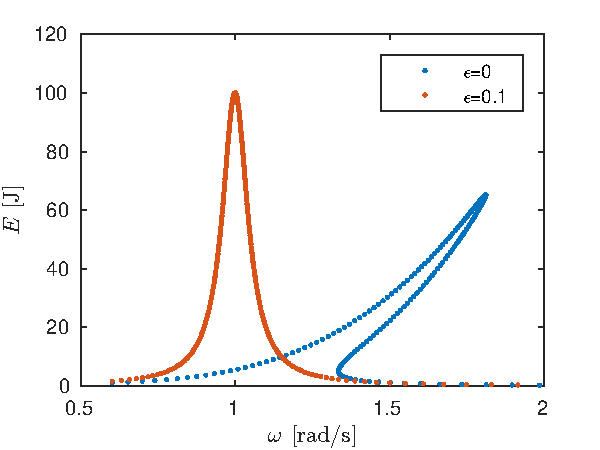
\includegraphics[scale=.75]{figure/continuation}
\caption{Energy-frequency plot}
\label{continuation}
\end{figure}

\begin{figure}[ht!]
	\centering
	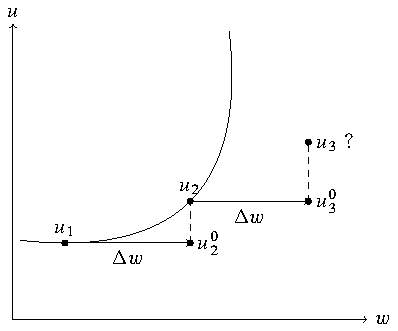
\includegraphics[scale=1]{figure/demo_parametric_continuation/tikz}
	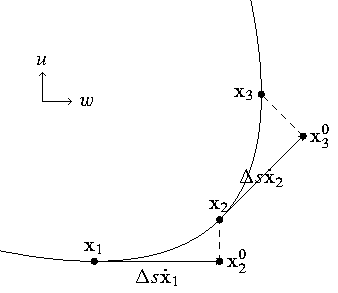
\includegraphics[scale=1]{figure/demo_arc-length_continuation/tikz}
	\caption{[Left] Demo of parametric continuation methods. [Right] Demo of arc-length continuation method. }
	\label{continuation/demo_arc-length_continuation}
\end{figure}

The idea of arclength continuation is quite illustrative by comparing the two figures in  Figure~\ref{continuation/demo_arc-length_continuation}. 
In the left figure, a implicit function with respect to $u$ and $w$ denotes the continuation curve. On the continuation curve $u_1$ is known and $u_2$ is to be solved. $\Delta w$ is the shift of parameter $w$. The idea of continuation is to solve $u_2$ given $w_2=w_1+\Delta w$. It demonstrates that the parametric continuation methods is not capable of finding $u_3$ given $u_2$ and $\Delta w$. It is not capable of tracing the curve through the turning point (also called the fold). 
In the right figure, vector $\mathbf x$ denotes $(u,w)^\top$. On the continuation curve $\mathbf x_1$ is known and $\mathbf x_2$ is to be solved. $\Delta s$ is the arc-length, $\dot{\mathbf x}_1$ is the normal direction of node $\mathbf x_1$. The idea of solving the node $\mathbf x_2$ is to solve the intersection between the continuation curve and the line $\mathbf x_2^0$-$\mathbf x_2$ which is orthogonal to the $\dot{\mathbf x}_1$. It demonstrates that the arc-length continuation methods is capable of overcoming the fold.

Given the solution $\mathbf u_0 \in \mathbb R^N$ and $w_0$ of a nonlinear (no differential term) equation $\mathbf f(\mathbf u,w): \mathbb R^{N+1} \rightarrow \mathbb R^{N}$, as well as the direction vector $\dot{\mathbf u}_0$ and $\dot{w}$, instead of moving the parameter variable $w$ by $w=w_0 +\Delta w$ which does not work of folders, a pseudo arc length $\Delta s$ is introduced, and move the solution along the curve for $\Delta s$. It still work when crossing a smooth folder where $\dot{w}=0$. 

Assume the curve is smooth, in the neighbour of $(\mathbf u_0, w_0)$, the curve can be approximated by Taylor expansion, and the initial guess of $(\mathbf u_1, w_1)$ can be predicted by 
\begin{equation}
\begin{aligned}
\mathbf u_1^{(0)} = \mathbf u_0 + \Delta s \dot{\mathbf u}_0
\\
w_1^{(0)} = w_0 + \Delta s \dot{w}_0
\end{aligned}
\end{equation}

Instead of solving nonlinear equation $f(\mathbf u_1)=0$ given a fixed $w_1$, we solve the augmented system where $f(\mathbf u_1,w_1)=0$ intersects with the line $(\mathbf u_1^{(0)}, w_1)$. Given $\Delta s$ small enough, and $f(\mathbf u_1)=0$ smooth enough, the solution is unique. 

The orthogonal line is formulated as
\begin{equation}
\begin{pmatrix}
\dot{\mathbf u}_0
&\dot{w}_0
\end{pmatrix}
\begin{pmatrix}
\mathbf u_1 -\mathbf u_1^{(0)}
\\w_1 -w_1^{(0)}
\end{pmatrix}
=0
\end{equation}

For normalized direction vector $\begin{pmatrix}\dot{\mathbf u}_0&\dot{w}_0\end{pmatrix}$, 
\begin{equation}
\begin{pmatrix}
\dot{\mathbf u}_0
&\dot{w}_0
\end{pmatrix}
\begin{pmatrix}
\mathbf u_1 -\mathbf u_0 - \Delta s \dot{\mathbf u}_0
\\w_1 -w_0 - \Delta s \dot{w}_0
\end{pmatrix}
=
\begin{pmatrix}
\dot{\mathbf u}_0
&\dot{w}_0
\end{pmatrix}
\begin{pmatrix}
\mathbf u_1 -\mathbf u_0 
\\w_1 -w_0 
\end{pmatrix}
- \Delta s 
\begin{pmatrix}
\dot{\mathbf u}_0
&\dot{w}_0
\end{pmatrix}
\begin{pmatrix}
\dot{\mathbf u}_0
\dot{w}_0
\end{pmatrix}
\end{equation}
\begin{equation}
\begin{pmatrix}
\dot{\mathbf u}_0
&\dot{w}_0
\end{pmatrix}
\begin{pmatrix}
\mathbf u_1 -\mathbf u_0 
\\w_1 -w_0 
\end{pmatrix}
- \Delta s
=0
\end{equation}

Define the augmented variable $\mathbf x=\begin{pmatrix} \mathbf u \\ w \end{pmatrix}$, 
The arclength continuation problem becomes solving $\mathbf f(\mathbf x_1)=0$. It can be solved with Newton-Raphson method. 

Given the Jacobian matrix (gradient matrix) $\mathbf f_{\mathbf x}$ at $\mathbf x_1$, the direction vector can be solved by considering that the direction vector is orthogonal to the gradient direction. 
\begin{equation}
\mathbf f_{\mathbf x_1} \dot{\mathbf x}_1 = \mathbf 0
\end{equation}
The solution is not unique cause $\mathbf f_{\mathbf x} : \mathbb R^{N+1} \rightarrow \mathbb R^N$. The graphic interpretation is that the length of the direction vector is undefined. We can get a unique solution by adding a normalization constraint
\begin{equation}
\dot{\mathbf x}_1^\top \dot{\mathbf x}_1 = 1
\end{equation}
However, the augmented solver for the direction is implicit
\begin{equation}
\begin{pmatrix}
\mathbf f_{\mathbf x} (\mathbf x_1)
\\\dot{\mathbf x}_1^\top 
\end{pmatrix}
\dot{\mathbf x}_1 = 
\begin{pmatrix}
\mathbf 0
\\1
\end{pmatrix}
\end{equation}
For $\mathbf f$ smooth enough and $\Delta s$ small enough, we assume $\dot{\mathbf x}_1 \approx \dot{\mathbf x}_0$, and solve it like this: 
\begin{equation}
\dot{\mathbf x}_1 = 
\begin{pmatrix}
\mathbf f_{\mathbf x} (\mathbf x_1)
\\\dot{\mathbf x}_0^\top 
\end{pmatrix}^{-1}
\begin{pmatrix}
\mathbf 0
\\1
\end{pmatrix}
\end{equation}
Before the extra normalization process.
\begin{equation}
\dot{\mathbf x}_1 
\leftarrow 
\frac{\dot{\mathbf x}_1 }{\Vert \dot{\mathbf x}_1 \Vert}
\end{equation}

\end{document}



